\documentclass[a4paper,12pt]{article}

\usepackage[slovene]{babel}
\usepackage{amsfonts,amssymb,amsmath}
\usepackage[utf8]{inputenc}
\usepackage[T1]{fontenc}
\usepackage{lmodern}
\usepackage{graphicx}
\usepackage{parskip}
\usepackage{wrapfig}

\newcommand{\geslo}[2]{\textbf{#1} \quad #2\newline}

\def\qed{$\hfill\Box$}   % konec dokaza
\def\qedm{\qquad\Box}   % konec dokaza v matematičnem načinu
\newtheorem{izrek}{Izrek}
\newtheorem{trditev}{Trditev}
\newtheorem{posledica}{Posledica}
\newtheorem{lema}{Lema}
\newtheorem{opomba}{Opomba}
\newtheorem{definicija}{Definicija}
\newtheorem{zgled}{Zgled}

\title{Kromatično število Kneserjevih grafov \\ 
\Large Seminar}
\author{Žan Hafner Petrovski \\
Fakulteta za matematiko in fiziko \\
Oddelek za matematiko}
\date{12.\ maj 2017}

\begin{document}

%%%%
 
\maketitle
\newpage

%%%%

\section{Uvod}

V teoriji grafov poznamo mnogo različnih tipov grafov. Razlikujemo jih glede na njihove specifične lastnosti. V tem seminarju se bomo ukvarjali s {\em Kneserjevimi grafi} oziroma podrobneje, s {\em kromatičnim številom} le-teh. Najprej podajmo nekaj glavnih definicij.

\begin{definicija}
Graf $K(n,k)$, $n \geq k \geq 1$ in $n, k \in \mathbb{N}$, imenujemo \mbox{\textbf{Kneserjev}}, če je množica vozlišč $V(n,k)$ družina vseh $k$-elementnih podmnožic množice $\{1, 2, \ldots, n\}$. Dve vozlišči sta povezani natanko takrat, ko sta disjunktni. 
\end{definicija}

V primeru, ko je $n < 2k$, imata vsaki dve $k$-elementni množici neprazen presek. Tak Kneserjev graf nima nobenih povezav, zato privzemimo, da velja $n \geq 2k$. 
Zdaj lahko še poenostavimo zapis in pišemo $n = 2k + d, k \geq 1, d \geq 0$.

\begin{definicija}
Preslikavo $c: V \rightarrow \{1, \ldots, m\}$, ki slika vozlišča grafa v množico barv, imenujemo \textbf {barvanje vozlišč grafa}. Barvanje vozlišč je pravilno, če sta vsaki dve sosednji vozlišči pobarvani z različnima barvama.
\end{definicija}

\begin{definicija}
Najmanjše naravno število $m$, za katero obstaja pravilno barvanje vozlišč grafa $G$ z $m$ barvami, imenujemo \textbf {kromatično število}. Označimo ga s $\chi(G).$
\end{definicija}

Kromatično število grafa $G$ je torej najmanjše število barv, s katerimi lahko pobarvamo vozlišča grafa tako, da nobeni sosednji vozlišči nista iste barve. 

Še nekoliko drugače povedano, množico vozlišč $V$ bi radi predstavili kot disjunktno unijo barvnih razredov, $V = V_1 \sqcup V_2 \sqcup \ldots \sqcup V_{\chi(G)}$, teh pa želimo, da je najmanj. 

Za vsak barvni razred velja, da imajo vsi njegovi elementi, torej $k$-elementne množice, neprazen presek. To sledi iz definicije Kneserjevih grafov, če bi imele te množice prazen presek, to je, obstajali bi vsaj dve disjunktni, med katerima bi obstajala povezava, zato pa bi bili pobarvani z različno barvo.

Omenimo še, da so Kneserjevi grafi posplošitev lihih grafov. Ti so namreč definirani kot grafi z $(n-1)$-elementnimi podmnožicami množice z $(2n-1)$ elementi, to pa se ujema z definicijo $K(2n-1,n-1)$.


\newpage
\section{Lastnosti Kneserjevih grafov}

V tem razdelku bomo opisali nekaj preprostejših lastnosti Kneserjevih grafov.

Najprej si oglejmo dva posebna primera. Prvi skrajni primer je, da za vsak $n \in \mathbb{N}$ velja, da je $K(n,1)$ poln graf, saj je vsaka točka svoje vozlišče in vsa vozlišča so disjunktna. Drugi pa, da je $K(2n,n)$ enak $\frac{1}{2} {{2n}\choose{n}}$ kopijam potnega grafa $P_2$. To je res, saj je vsaka $n$-elementna podmnožica v $\{1,\ldots,2n\}$ disjunktna le s svojim komplementom.

\begin{figure}[h!]
\centering
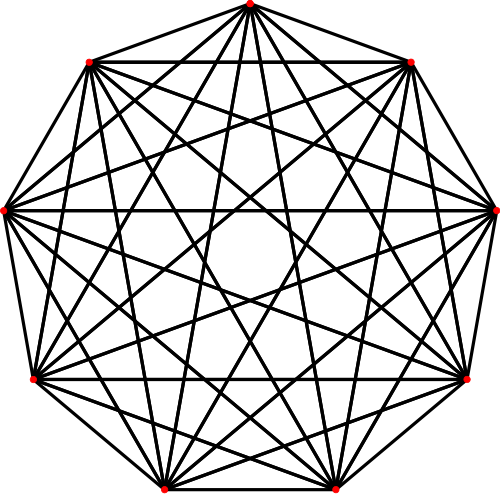
\includegraphics[width=0.2\textwidth]{poln_graf}
\caption{Poln graf $K_9=K(9,1)$}
\end{figure}

Hitro vidimo, da za število vozlišč velja $|V(n,k)|={{n}\choose{k}}$. Malenkost manj očitno je, da je graf regularen. Njegovo stopnjo lahko izračunamo, če iz množice z $n$ elementi odstranimo $k$ elementov, ki jih vsebuje vsako vozlišče, potem pa jih iz preostalih $n-k$ izberemo $k$, ki jih vsebuje vozlišče, s katerim je povezano prvotno vozlišče. Takih povezav lahko za vsako vozlišče tvorimo ravno ${n-k}\choose{k}$, kar je stopnja regularnosti grafa.


\begin{zgled}{Kneserjev graf $K(5,2)$ je zelo znan primer, imenujemo ga Petersenov graf. 

\begin{figure}[h!]
	\centering
	\begin{minipage}{0.45\textwidth}
		\centering
		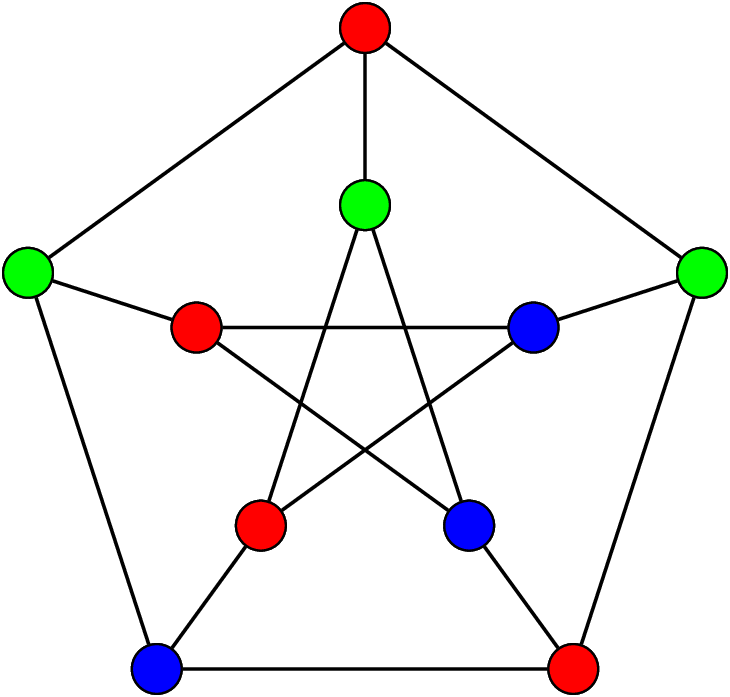
\includegraphics[width=0.8\textwidth]{petersenov_graf_barvanje}
        	\caption{Primer barvanja tega grafa z $d+2$, torej $3$ barvami}
    	\end{minipage}\hfill
    	\begin{minipage}{0.45\textwidth}
       	 \centering
        	 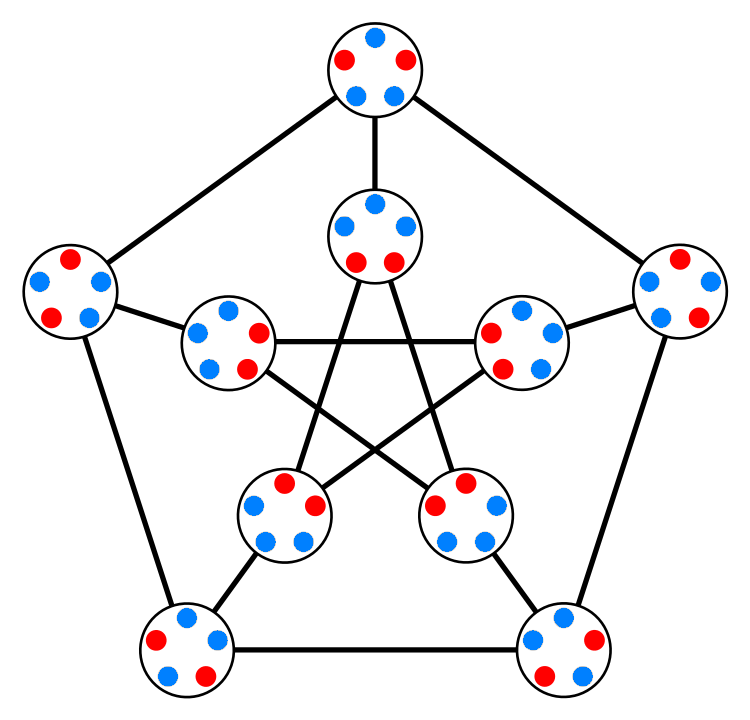
\includegraphics[width=0.8\textwidth]{petersenov_graf_mnozice}
       	 \caption{Prikaz povezav med disjunktnimi množicami}
    	\end{minipage}
\end{figure}

Ta graf zelo pogosto pride prav pri dokazovanju obstoja nekega tipa grafa ali pa kot protiprimer. Imenuje se po Juliusu Petersenu, ki ga je skonstruiral za najmanjši kubični graf, to je, graf, ki je regularen stopnje $3$, brez mostov in brez barvanja robov s tremi barvami. Ima $10$ vozlišč in $15$ povezav, kar se ujema s prej opisanima lastnostima.}

\end{zgled}



Da dobimo idejo, s koliko barvami zanesljivo lahko pobarvamo Kneserjev graf, si oglejmo naslednjo trditev.

\begin{trditev}
Vozlišča Kneserjevega grafa $K(2k+d,k)$ lahko pobarvamo z $d+2$ barvama.
\end{trditev}

\noindent
{\em Dokaz:}
Zapišimo preprost predpis za barvanje grafa $K(2k+d,k)$, pri katerem uporabimo $d+2$ barv. Za števila $i$ iz $\{1,2,\ldots,d+1\}$ naj množica $V_i$ sestoji iz vseh $k$-elementnih podmnožic, ki imajo $i$ za najmanjši element. Preostale \mbox{$k$-elementne} podmnožice so vsebovane v množici $\{d+2,d+3,\ldots,2k+d\}$, katere moč je le $2k-1$. Sledi, da imajo te množice neprazen presek in lahko zanje uporabimo barvo $d+2$.\qed

Tako smo dobili $\chi(K(2k+d,k)) \leq d+2$. Kneser je postavil domnevo, da je $d+2$ kar najmanjše možno število barv, torej kromatično število Kneserjevega grafa $K(2k+d,k)$ je $d+2$.

\newpage

\section{Kneserjeva domneva}

Cilj tega seminarja je dokazati naslednji izrek:
\begin{izrek}[Kneser]
Za kromatično število Kneserjevega grafa velja
$$\chi(K(2k+d,k)) = d+2.$$
\end{izrek}

\noindent
Preformulirajmo ta izrek v obliko problema obstoja na sledeč način:

\begin{izrek}[Ekvivalenten Kneserjevemu izreku]
Če družino $k$-elementnih podmnožic množice $\{1, 2, \ldots, 2k+d\}$ razdelimo na $d+1$ razredov,  $V = V_1 \sqcup V_2 \sqcup \ldots \sqcup V_{d+1}$, potem obstaja $i$ tako, da $V_i$ vsebuje par disjunktnih $k$-elementnih množic $A$ in $B$.
\end{izrek}

V jeziku grafov to pomeni, da bi z isto barvo pobarvail sosednji vozlišči. Ta različica izreka nam, še preden se poglobimo v sam dokaz, nudi drugačen pogled na zastavljen problem, saj ne omenja grafov. Želimo le pokazati obstoj množic $A$ in $B$. László Lovász je uvidel, da bistvo problema tiči v slavnem izreku o $d$-dimenzionalni enotski sferi $S^d$ v $\mathbb{R}^{d+1}$, $S^d = \{x \in \mathbb{R}: |x|=1\}$. Zapišimo še ta izrek.

\begin{izrek}[Borsuk-Ulam]
Za vsako zvezno preslikavo $f:S^d \rightarrow \mathbb{R}^d$ $d$-sfere v $d$-prostor, obstajata antipodni točki $x^*$ in $-x^*$, ki ju $f$ slika v isto točko, torej $f(x^*)=f(-x^*)$.
\end{izrek}

Dokaz tega izreka lahko bralec najde v knjigi ''Using the Borsuk-Ulam theorem'' matematika Jirija Matouška, mi pa se bomo posvetili njegovi uporabi pri dokazu izreka Lyusternika in Shnirel'mana.

\begin{izrek}[Lyusternik-Shnirel'man]
Če je $d$-sfera $S^d$ pokrita z $d+1$ množicami,
$$S^d = U_1 \cup U_2 \cup \ldots \cup U_d \cup U_{d+1},$$
tako, da je vsaka izmed prvih $d$ množic $U_1, U_2, \ldots, U_d$ bodisi odprta bodisi zaprta, potem ena izmed $d+1$ množic vsebuje par antipodnih točk $x^*$ in $-x^*$.
\end{izrek}

Za dokaz Kneserjeve domneve potrebujemo le primer, ko so $U_1, \ldots, U_d$ odprte, vseeno pa je naveden splošnejši izrek, ki od množic zahteva le odprtost ali pa zaprtost. Iz dokaza je razvidno, da odprtost in zaprtost uporabimo vsakič le za posamezno množico.

\newpage
\begin{zgled}{Za občutek si oglejmo sfero $S^1$ pokrito z $d+1$, torej z $2$ množicama. Množica $A$, ki je na sliki narisana z zvezno krivuljo, je odprta, $B$, ki je narisana črtkano, pa poljubna taka, da velja $A \cup B = S^1$. V tem primeru je očitno, da $B$ vsebuje antipodni točki. 
\begin{figure}[h!]
\centering
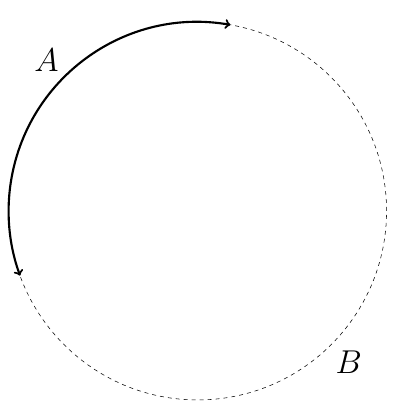
\includegraphics[width=0.27\textwidth]{sfera_s1}
\caption{Sfera $S^1$}
\end{figure}
}
\end{zgled}


\noindent
{\em Dokaz s protislovjem in uporabo Borsuk-Ulamovega izreka:} \\
\indent Naj bo pokritje $S^d = U_1 \cup U_2 \cup \ldots \cup U_d \cup U_{d+1}$ dano, kot je zapisano v izreku. Predpostavimo, da noben izmed $U_i$ ne vsebuje dveh antipodnih točk. 

Definirajmo preslikavo $f:S^d \rightarrow \mathbb{R}^d$ na sledeč način:
$$f(x) := (d(x,U_1), d(x,U_2), \ldots, d(x,U_d)).$$

Tu $d(x,U_i)$ označuje razdaljo med točko $x$ in množico $U_i$. Ker je to zvezna funkcija na $x$, je tudi $f$ zvezna. Torej lahko uporabimo Borsuk-Ulamov izrek, ki nam pove, da na domeni $f$, torej na $S^d$, obstajata antipodni točki $x^*$ in $-x^*$ z lastnostjo $f(x^*)=f(-x^*)$. Ker po predpostavki z začetka dokaza $U_{d+1}$ ne vsebuje antipodnih točk, sklepamo, da je vsaj en izmed $x^*$ in $-x^*$ vsebovan v eni izmed množic $U_i$, recimo v $U_k$ za $k\leq d$. Brez škode za splošnost lahko privzamemo, da je to $x^*$, torej $x^* \in U_k$. To pomeni, da je $d(x^*, U_k) = 0$, ključno pa je, da je zaradi lastnosti $f(x^*)=f(-x^*)$ tudi $d(-x^*, U_k) = 0$.

Obravnavajmo najprej primer, ko je $U_k$ zaprt. Potem iz $d(-x^*, U_k) = 0$ sledi, da je $-x^* \in U_k$, kar pa je protislovje s predpostavko, da noben izmed $U_i$ ne vsebuje para antipodnih točk.

Če je $U_k$ odprt, potem iz $d(-x^*, U_k) = 0$ sledi, da $-x^*$ leži v zaprtju $U_k$, torej v $\overline U_k$. Ta množica pa je vsebovana v $S^d\textbackslash(-U_k)$, \mbox{$-U_k = \{-x;x \in U_k\}$}. Množica $S^d\textbackslash(-U_k)$ je namreč zaprta in vsebuje $U_k$, pri tem smo upoštevali predpostavko, da $U_k$ ne vsebuje antipodnih točk. Ampak, ker je zaprta in vsebuje $U_k$, vsebuje tudi $\overline U_k$. To pomeni, da $-x^*$ leži v  $S^d\textbackslash(-U_k)$, torej ne more ležati v $-U_k$. Ker pa smo privzeli, da $x^* \in U_k$, smo prišli do protislovja.\qed 
\newpage

V svojem dokazu iz leta 1978 je Imre Bárány uporabil še Galeov izrek o obstoju določene postavitve točk na sfero $S^d$. Bárány je svoj dokaz objavil nekaj tednov za tem, ko je László Lovász prvi dokazal Kneserjevo domnevo s pomočjo Borsuk-Ulamovega dokaza.

\begin{izrek}[Gale]
Za vsak $d \geq 0$ in vsak $d \geq 1$ obstaja taka postavitev $2k+d$ točk na $d$-dimenzionalno sfero $S^d$, da vsaka odprta polsfera vsebuje vsaj $k$ izmed teh točk.
\end{izrek}

Tudi dokaz tega izreka lahko bralec najde v Matouškovi knjigi ''Using the Borsuk-Ulam theorem''. Dokaz ni tako preprost, zato je še večjega pomena Greenova poenostavitev Bárányjevega dokaza. Leta 2002 je Joshua Greene namreč ugotovil, da zadošča, če so točke iz izreka v splošni legi na sferi. Tu je zapisan njegov dokaz.

\begin{definicija}
Točke iz množice $\{1,2,\ldots,2k+d\}$ so v \textbf {splošni legi} na sferi $S^{d+1} \subset \mathbb{R}^{d+2}$, če nobenih $d+2$ točk iz omenjene množice ne leži na hiperravnini skozi središče sfere.
\end{definicija}

\begin{figure}[h!]
\centering
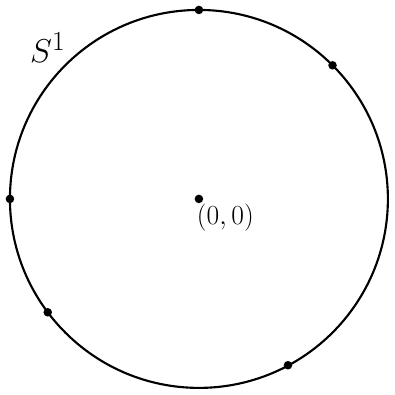
\includegraphics[width=0.35\textwidth]{splosna_lega}
\caption{Primer za $d=0$, postavitev $4$ točk sfero $S^1$}
\end{figure}


\noindent
{\em Dokaz Kneserjeve domneve:}\\
\indent Vzemimo množico točk $\{1,2,\ldots,2k+d\}$ in jih postavimo v splošno lego na sfero $S^{d+1}$. Naj bo $V(n,k)$ družina vseh $k$-elementnih podmnožic začetne množice, razdelimo jo na $d+1$ razredov, $V(n,k) = V_1 \sqcup V_2 \sqcup \ldots \sqcup V_{d+1}$. Naš cilj je najti par disjunktnih $k$-elementnih množic $A$ in $B$, ki pripadata istemu razredu $V_i$.
\newpage


Za $i=1, 2,\ldots, d+1$ definirajmo
\begin{align*} O_i = \{x \in S^{d+1}; &\text{ odprta polsfera } H_x \text{ z vrhom } x \\ &\text{ vsebuje } k\text{-elementno množico iz } V_i\}.
\end{align*}

\begin{figure}[h]
\centering
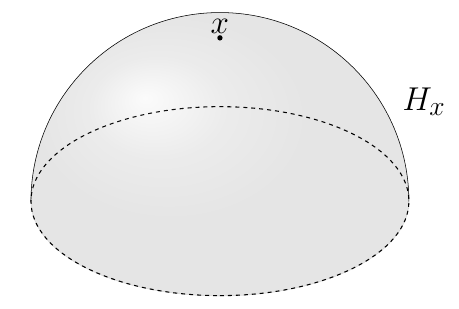
\includegraphics[width=0.35\textwidth]{polsfera}
\end{figure}


Vsaka množica $O_i$ je odprta. Za vsak $x \in O_i$ namreč obstaja neka odprta okolica, za vsak element $y$ iz te okolice pa še vedno velja, da polsfera, katere vrh je $y$, vsebuje istih $k$-elementov kot polsfera, katere vrh je $x$. To sledi iz dejstva, da smo v definiciji množic $O_i$ uporabili {\em odprte} polsfere.

Odprte množice $O_i$ in zaprta množica $C = S^{d+1} \backslash (O_1 \cup \ldots \cup O_{d+1})$ tvorijo pokritje $S^{d+1}$. To pokritje zadošča pogoju iz izreka Lyusternik-Shnirel'mana, zato vemo, da ena izmed množic iz omenjenega pokritja vsebuje antipodni točki $x^*$ in $-x^*$. 

To ne more biti množica $C$, saj po definiciji polsferi $H_{x^*}$ in $H_{-x^*}$, ko velja $x^*, -x^* \in C$, vsebujeta manj kot $k$ točk. To je res, saj unija množic $O_i$ vsebuje {\em vse} vrhove polsfer, ki vsebujejo $k$-elementne podmnožice začetne množice, $C$ pa je komplement te unije. Sledi, da vsaj $d+2$ točki ležita na ekvatorju $\overline H_{x^*} \cap \overline H_{-x^*}$, torej na hiperravnini skozi središče sfere. To pa ne more biti res, saj so točke v splošni legi.

Zato ena izmed množic $O_i$ vsebuje antipodni točki $x^*$ in $-x^*$. Po definiciji množic $O_i$  obstajata \mbox{$k$-elementni} množici $A, B \in V_i$ z lastnostjo $A \subseteq H_{x^*}$ in $B \subseteq H_{-x^*}$. 

Ker pa govorimo o {\em odprtih} polsferah, sta $H_{x^*}$ in $H_{-x^*}$ disjunktni. Sledi, da sta tudi $A$ in $B$ disjunktni. Našli smo torej disjunktni $k$-elementni množici, ki pripadata istemu razredu množic $V_i$. \qed


%%%%
\newpage

\section*{Angleško-slovenski slovar strokovnih izrazov}

\geslo{Kneser graph}{Kneserjev graf}
\geslo{graph coloring}{barvanje grafa}
\geslo{chromatic number}{kromatično število}
\geslo{unit sphere}{enostka sfera}
\geslo{antipodal points}{antipodni točki}
\geslo{covering}{pokritje}
\geslo{general position}{splošna lega}
\geslo{hemisphere}{polsfera}
\geslo{hyperplane}{hiperravnina}
\geslo{equator}{ekvator}

\begin{thebibliography}{1}

\bibitem{AiZ}
M.~Aigner in G.~M.~Ziegler, \emph{Proofs from THE BOOK}, 4.\ izdaja, Springer, Berlin--Heidelberg--New York, 2010.
\bibitem{JiM}
J.~Matoušek, \emph{Using the Borsuk-Ulam theorem}, Springer-Verlag Berlin Heidelberg, 2003.
%https://math.berkeley.edu/{tu manjka ~}brandtm/research/kneser.pdf (25.4.2017)
%http://oai.cwi.nl/oai/asset/9898/9898A.pdf
%https://en.wikipedia.org/wiki/Petersen_graph (10.5.2017)

%slike
%https://graphtheoryinlatex.files.wordpress.com/2010/02/coloringpeteresen2.png
%http://blogs.ams.org/visualinsight/files/2015/06/petersen_graph.png
\end{thebibliography}

\end{document}